\section*{Seminár 10}
\subsection*{Téma}
Geometria II -- podobné trojuholníky a Pytagorova veta

\subsection*{Ciele}
Precvičiť riešenie úloh vhodným (viacnásobným) využitím Pytagorovej vety a dvojíc podobných trojuholníkov

\subsection*{Úlohy a riešenia}
\begin{tcolorbox}[breakable,notitle,boxrule=0pt,colback=light-gray,colframe=light-gray]\ul{10.1} [66-S-3] Päta $P$ výšky z~vrcholu $C$ v~trojuholníku $ABC$ delí stranu $AB$ v~pomere $|AP| : |PB|= 1 : 3$. V~rovnakom pomere sú aj obsahy štvorcov nad jeho stranami $AC$ a $BC$.
Dokážte, že trojuholník $ABC$ je pravouhlý.
\end{tcolorbox}

\rieh Označme $d$ dĺžku úsečky $AP$ a $v$ dĺžku výšky $CP$ trojuholníka $ABC$. Dĺžky jeho strán označíme zvyčajným spôsobom $a, b, c$. Zo zadania teda vyplýva $|PB| = 3d$.
\begin{center}
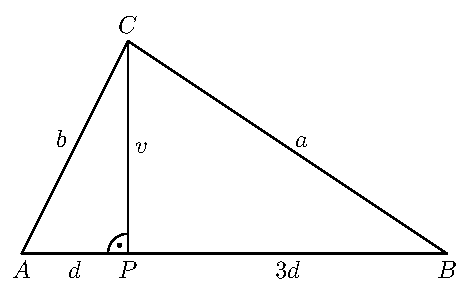
\includegraphics{obrazky/66S3.pdf}\\

Obr. 1
\end{center}
Použitím Pytagorovej vety v~trojuholníkoch $APC$ a $PBC$ dostávame rovnosti $b^2= d^2 +v^2$ a $a^2 = 9d^2 +v^2$. Z~druhého predpokladu úlohy potom vyplýva rovnosť $a^2 = 3b^2$, čiže $9d^2 + v^2 = 3d^2 + 3v^2$, odkiaľ $v^2 = 3d^2$. Dosadením do prvých dvoch rovností tak dostávame $a^2 = 12d^2$ a $b^2 = 4d^2$. A~keďže $c = 4d$, čiže $c^2 = 16d^2$, dokázali sme, že pre dĺžky strán trojuholníka $ABC$ platí $a^2 + b^2 = c^2$.

Trojuholník $ABC$ je preto podľa obrátenej Pytagorovej vety pravouhlý.\\
\\
\textit{Poznámka.} Ak zvážime pomocný pravouhlý trojuholník s~odvesnami $a$ a $b$, tak pre jeho preponu~$c'$ podľa Pytagorovej vety platí $c' = a^2 + b^2$. Porovnaním s~odvodenou rovnosťou $c^2 = a^2 + b^2$ tak dostávame $c'= c$, takže pôvodný trojuholník je podľa vety $sss$ zhodný s~trojuholníkom pomocným, a je teda skutočne pravouhlý. Môžeme tolerovať názor, že samotná Pytagorova veta udáva nielen nutnú, ale aj postačujúcu podmienku na to, aby bol daný trojuholník pravouhlý.\\
\\
\kom Úloha relatívne priamočiaro využíva viacnásobné využitie Pytagorovej vety, je tak vhodným zahrievacím problémom tohto seminára.\\
\\
\begin{tcolorbox}[breakable,notitle,boxrule=0pt,colback=light-gray,colframe=light-gray]\ul{10.2} [66-I-3]
Päta výšky z~vrcholu $C$ v~trojuholníku $ABC$ delí stranu $AB$ v~pomere $1 : 2$. Dokážte, že pri zvyčajnom označení dĺžok strán trojuholníka $ABC$ platí nerovnosť $$3|a - b| < c.$$
\end{tcolorbox}

\rieh Päta $D$ uvažovanej výšky je podľa zadania tým vnútorným bodom strany $AB$, pre ktorý platí $|AD| = 2|BD|$ alebo $|BD| = 2|AD|$. Obe možnosti sú znázornené na obr.\,2 s~popisom dĺžok strán $AC$, $BC$ a oboch úsekov rozdelenej strany $AB$.
\begin{center}
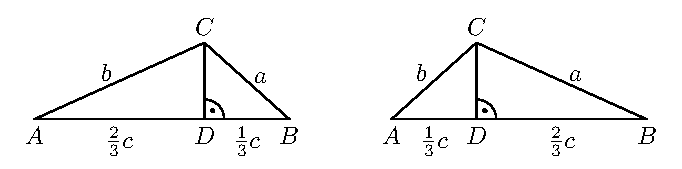
\includegraphics{obrazky/66D31.pdf}\\

Obr. 2
\end{center}
Pytagorova veta pre pravouhlé trojuholníky $ACD$ a $BCD$ vedie k~dvojakému vyjadreniu druhej mocniny spoločnej odvesny $CD$, pričom v~situácii naľavo dostaneme
$$|CD|^2= b^2- \bigg(\frac{2}{3}c\bigg)^2= a^2 - \bigg(\frac{1}{3}c\bigg)^2,$$
odkiaľ po jednoduchej úprave poslednej rovnosti dostaneme vzťah
$$3(b^2 - a^2) = c^2.$$
Pre druhú situáciu vychádza analogicky
$$3(a^2 -b^2) = c^2.$$
Závery pre obe možnosti možno zapísať jednotne ako rovnosť s~absolútnou hodnotou
$$3|a^2 - b^2 | = c^2.$$
Ak použijeme rozklad $|a^2 - b^2 | = |a - b|(a + b)$ a nerovnosť $c < a + b$ (ktorú ako je známe spĺňajú dĺžky strán každého trojuholníka $ABC$), dostaneme z~odvodenej rovnosti
$$3|a - b|c < 3|a - b|(a + b) = c^2,$$
odkiaľ po vydelení kladnou hodnotou $c$ dostaneme $3|a - b| < c$, ako sme mali dokázať. Zdôraznime, že nerovnosť $3|a-b|c < 3|a-b|(a+b)$ sme správne zapísali ako ostrú -- v~prípade $a = b$ by síce prešla na rovnosť, avšak podľa nášho odvodenia by potom platilo $c^2 = 0$, čo odporuje tomu, že ide o~dĺžku strany trojuholníka.\\
\\
\textbf{Iné riešenie.} Nerovnosť, ktorú máme dokázať, možno po vydelení tromi zapísať bez
absolútnej hodnoty ako dvojicu nerovností
$$-\frac{1}{3}c < a - b < \frac{1}{3}c.$$
Opäť ako v~pôvodnom riešení rozlíšime dve možnosti pre polohu päty $D$ uvažovanej výšky a ukážeme, že vypísanú dvojicu nerovností možno upresniť na tvar
$$-\frac{1}{3} < a - b < 0,\ \ \ \ \text{respektíve} \ \ \ \  0 < a - b <\frac{1}{3}c,$$
podľa toho, či nastáva situácia z~ľavej či pravej časti obr. 2.

Pre situáciu z~obr. 2 naľavo prepíšeme avizované nerovnosti $-\frac{1}{3}c < a - b < 0$ ako $a < b < a +\frac{1}{3}c$ a odvodíme ich z~pomocného trojuholníka $ACE$, pričom $E$ je stred úsečky $AD$, takže body $D$ a $E$ delia stranu $AB$ na tri zhodné úseky dĺžky $\frac{1}{3}c$.
\begin{center}
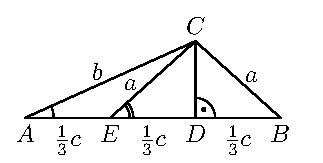
\includegraphics{obrazky/66D32}\\

Obr. 3
\end{center}
V~obr. 3 sme rovno vyznačili, že úsečka $EC$ má dĺžku $a$ ako úsečka $BC$, a to v~dôsledku zhodnosti trojuholníkov $BCD$ a $ECD$ podľa vety $sus$. Preto je pravá z~nerovností $a < b < a +\frac{1}{3}c$ porovnaním dĺžok strán trojuholníka $ACE$, ktoré má všeobecnú platnosť.

Ľavú nerovnosť $a < b$ odvodíme z~druhého všeobecného poznatku, že totiž v~každom trojuholníku oproti väčšiemu vnútornému uhlu leží dlhšia strana. Stačí nám teda zdôvodniť, prečo pre uhly vyznačené na obr. 3 platí $|\ma CAE| < |\ma AEC|$. To je však jednoduché: zatiaľ čo uhol $CAE$ je vďaka pravouhlému trojuholníku $ACD$ ostrý, uhol $AEC$ je naopak tupý, pretože k~nemu vedľajší uhol $CED$ je ostrý vďaka pravouhlému trojuholníku $CED$.

Pre prípad situácie z~obr. 2 napravo možno predchádzajúci postup zopakovať s~novým bodom $E$, tentoraz stredom úsečky $BD$. Môžeme však vďaka súmernosti podľa osi $AB$ konštatovať, že z~dokázaných nerovností $-\frac{1}{3}c < a - b < 0$ pre situáciu naľavo vyplývajú nerovnosti $-\frac{1}{3}c < b - a < 0$ pre situáciu napravo, z~ktorých po vynásobení číslom $-1$ dostaneme práve nerovnosti $0 < a - b <\frac{1}{3}$, ktoré sme mali v~druhej situácii dokázať.\\
\\
\kom Nosným prvkom úlohy je opäť Pytagorova veta, väčšiu pozornosť však vyžaduje rozbor úlohy, keďže päta výšky sa môže nachádzať v~dvoch rôznych polohách.\\
\\
\begin{tcolorbox}[breakable,notitle,boxrule=0pt,colback=light-gray,colframe=light-gray]\ul{10.3} [63-S-3]
Daný je trojuholník $ABC$ s~pravým uhlom pri vrchole $C$. Stredom $I$ kružnice trojuholníku vpísanej vedieme rovnobežky so stranami $CA$ a $CB$, ktoré pretnú preponu postupne v~bodoch $X$ a $Y$. Dokážte, že platí $|AX|^2 + |BY |^2 = |XY |^2$.

\end{tcolorbox}

\rieh Trojuholník $AIX$ je rovnoramenný, pretože $|\ma IAX| = |\ma IAC| = | \ma AIX|$ (prvá rovnosť vyplýva z~podmienky, že bod $I$ leží na osi uhla $BAC$, druhá potom z~vlastností striedavých uhlov, obr. 4). Preto $|AX| = |IX|$. Analogicky zistíme, že $|BY | = |Y I|$. Keďže úsečky $IX$ a $IY$ zvierajú (rovnako ako s~nimi rovnobežné úsečky $CA$ a $CB$) pravý uhol, podľa Pytagorovej vety pre pravouhlý trojuholník $XIY$ platí $$|AX|^2+ |BY |^2= |IX|^2+ |Y I|^2= |XY |^2,$$
čo sme mali dokázať.
\begin{center}
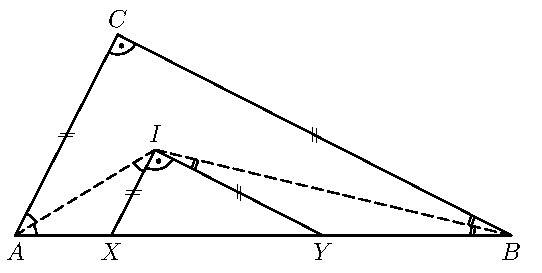
\includegraphics{obrazky/63S3}\\

Obr. 4
\end{center}
\kom Úloha už vyžaduje trochu viac invencie a postrehu, keďže kľúčovým krokom v~riešení je všimnúť si, že trojuholníky $AIX$ a $BIY$ sú rovnoramenné. K~tomu však študentov môže naviesť poloha bodu $I$, ktorý leží na osi uhlov a to, že rovnobežky $AC$ a $XI$, resp. $BC$ a $YI$ sú preťaté priečkami $AI$, resp. $BI$, takže v~náčrtku vieme nájsť niekoľko dvojíc zhodných uhlov. Úloha tak kombinuje použitie Pytagorovej vety aj vlastnosti rovnoramenných trojuholníkov.\\
\\
\begin{tcolorbox}[breakable,notitle,boxrule=0pt,colback=light-gray,colframe=light-gray]\ul{10.4} [58-S-2]
 V~pravouhlom trojuholníku $ABC$ označíme $P$ pätu výšky z~vrcholu $C$ na preponu $AB$. Priesečník úsečky $AB$ s~priamkou, ktorá prechádza vrcholom $C$ a stredom kružnice vpísanej trojuholníku $PBC$, označíme $D$. Dokážte, že úsečky $AD$ a $AC$ sú zhodné.

\end{tcolorbox}

\rieh V~pravouhlom trojuholníku $ABC$ s~preponou $AB$ pre veľkosti $\alpha, \beta$ uhlov pri vrcholoch $A$, $B$ platí $\alpha+\beta= 90^\circ$, preto $|\ma ACP| = 90^\circ -\alpha = \beta$ a $|\ma BCD| = | \ma DCP|= \frac{1}{2}(90^\circ -\beta) = \frac{1}{2}\alpha$ lebo priamka $CD$ je osou uhla $BCP$ (obr. 5). Pre vonkajší uhol $ADC$ trojuholníka $BCD$ tak zrejme platí $|\ma ADC| = |\ma DBC| + |\ma BCD| = \beta  +\frac{1}{2}\alpha = |\ma DCA|.$

Zistili sme, že trojuholník $ADC$ má pri vrcholoch $C, D$ zhodné vnútorné uhly, je
teda rovnoramenný, a preto $|AD| = |AC|$.
\begin{center}
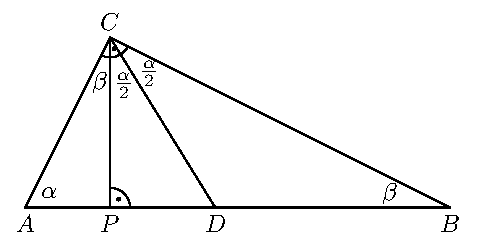
\includegraphics{obrazky/58S21}\\

Obr. 5
\end{center}
\kom Úloha je zameraná na nájdenie veľkosti vhodných uhlov\footnote{V anglickej literatúre sa tejto metóde -- počítaniu veľkostí všemožných uhlov -- hovorí \textit{angle-chasing}.} a využitie poznatku, že uhly pri základni rovnoramenného trojuholníka majú rovnakú veľkosť.\\
\\
\begin{tcolorbox}[breakable,notitle,boxrule=0pt,colback=light-gray,colframe=light-gray]\ul{10.5} [64-I-4] Označme $E$ stred základne $AB$ lichobežníka $ABCD$, v~ktorom platí $|AB| : |CD| = 3 : 1$. Uhlopriečka $AC$ pretína úsečky $ED$, $BD$ postupne v~bodoch $F$, $G$. Určte postupný pomer $|AF| : |FG| : |GC|$.

\end{tcolorbox}

\rieh  Keďže v~zadaní aj v~otázke úlohy sú iba pomery, môžeme si dĺžky strán lichobežníka zvoliť ako vhodné konkrétne čísla. Zvoľme teda napr. $|AB| = 6$, potom $|AE| = |BE| = 3$ a $|CD| = 2$. Hľadané dĺžky označme $|AF| = x$, $|FG| = y$, $|GC| = z$. Tieto dĺžky sme vyznačili na obr. 6, taktiež aj tri dvojice zhodných uhlov, ktoré teraz využijeme pri úvahách o~trojuholníkoch podobných podľa vety $uu$.

Trojuholníky $ABG$ a $CDG$ sú podobné, preto $(x + y) : z~= 6 : 2 = 3 : 1$. Aj trojuholníky $AEF$ a $CDF$ sú podobné, preto $x : (y + z) = 3 : 2$.
\begin{center}
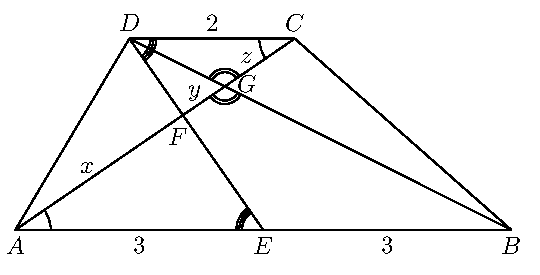
\includegraphics{obrazky/64D4}\\
Obr. 6
\end{center}
Odvodené úmery zapíšeme ako sústavu rovníc
\begin{align*}
x + y - 3z &= 0,\\
2x - 3y - 3z &= 0.
\end{align*}
Ich odčítaním získame rovnosť $x = 4y$, čiže $x : y = 4 : 1$. Dosadením tohto výsledku do prvej rovnice dostaneme $5y = 3z$, čiže $y : z~= 3 : 5$. Spojením oboch pomerov získame výsledok $x : y : z~= 12 : 3 : 5$.\\
\\
\kom Úloha je výborným tréningom na hľadanie vhodných dvojíc podobných trojuholníkov tak, aby sme pomocou údajov zo zadania boli schopní určiť hľadaný pomer, keďže jedna dvojica trojuholníkov na nájdenie odpovede zjavne stačiť nebude. Okrem toho tiež pozorovania z~náčrtu vedú k~sústave dvoch rovníc, takže študenti uplatnia aj svoje algebraické zručnosti.\\
\\
\begin{tcolorbox}[breakable,notitle,boxrule=0pt,colback=light-gray,colframe=light-gray]\ul{10.6} [63-I-4] Vo štvorci $ABCD$ označme $K$ stred strany $AB$ a $L$ stred strany $AD$. Úsečky $KD$ a $LC$ sa pretínajú v~bode $M$ a rozdeľujú štvorec na dva trojuholníky a dva štvoruholníky. Vypočítajte ich obsahy, ak úsečka $LM$ má dĺžku 1\,cm.

\end{tcolorbox}

\rieh Platí $|AK| = |DL|$ a $|AD| = |DC| = 2|AK|$ (obr. 7), takže pravouhlé trojuholníky $AKD$ a $DLC$ sú zhodné podľa vety $sus$. Okrem toho sú trojuholníky $MLD$ a $AKD$ podobné podľa vety $uu$, lebo $|\ma LDM| = |\ma KDA|$ a $|\ma DLM| = |\ma DLC| = |\ma AKD|$. Analogicky sa dá overiť i podobnosť trojuholníkov $MDC$ a $AKD$. Z~podobnosti trojuholníkov $AKD$, $MLD$ a $MDC$ vyplýva, že $|MD| = 2|ML| = 2$\,cm a $|MC| = 2|MD| = 4$\,cm. Obsahy útvarov $MLD$, $MDC$ a $AKML$ sú
$$S_{MLD} =\frac{1\cdot 2}{2}= 1\,\text{cm}^2, \ \ \ \  S_{MDC} = \frac{2\cdot 4}{2}= 4\,\text{cm}^2$$
a
$$S_{AKML} = S_{AKD}- S_{MLD} = S_{DLC} - S_{MLD} = S_{MDC} = 4\,\text{cm}^2.$$
Nakoniec pomocou Pytagorovej vety dostávame $S_{ABCD} = |DC|^2 = |DM|^2 + |CM|^2= 20$\,cm$^2$, takže
$$S_{KBCM} = S_{ABCD} - (S_{MLD} + S_{MDC} + S_{AKML}) = 11\,\text{cm}^2.$$
\textit{Záver.} Obsahy trojuholníkov $MLD$, $MDC$ a štvoruholníkov $AKML$, $KBCM$ sú postupne 1\,cm$^2$, 4\,cm$^2$, 4\,cm$^2$ a 11\,cm$^2$.
\begin{center}
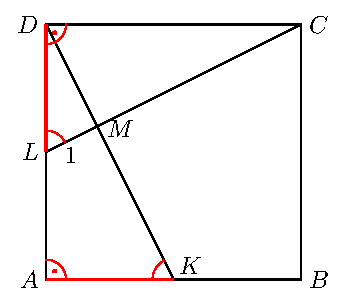
\includegraphics{obrazky/63D41}

Obr. 7
\end{center}
\kom Opäť je potrebné identifikovať podobné trojuholníky a potom pomocou známeho koeficientu určiť ich obsahy. Oproti predchádzajúcej úlohe ešte študenti navyše využijú Pytagorovu vetu.\\
\\
\begin{tcolorbox}[breakable,notitle,boxrule=0pt,colback=light-gray,colframe=light-gray]\ul{10.7} [65-II-3] V~pravouhlom lichobežníku $ABCD$ s~pravým uhlom pri vrchole $A$ základne $AB$ je bod $K$ priesečníkom výšky $CP$ lichobežníka s~jeho uhlopriečkou $BD$. Obsah štvoruholníka $APCD$ je polovicou obsahu lichobežníka $ABCD$. Určte, akú časť obsahu trojuholníka $ABC$ zaberá trojuholník $BCK$.

\end{tcolorbox}

\rieh V~pravouholníku $APCD$ označme $c = |CD| = |AP|$ a $v = |AD| = |CP|$ (obr.~8, pričom sme už vyznačili ďalšie dĺžky, ktoré odvodíme v~priebehu riešenia)\footnote{Keďže podľa zadania uhlopriečka $BD$ pretína výšku $CP$, musí jej päta $P$ ležať medzi bodmi $A$ a $B$, takže ide o~\uv{zvyčajný} lichobežník $ABCD$ s~dlhšou základňou $AB$ a kratšou základňou $CD$.}.
\begin{center}
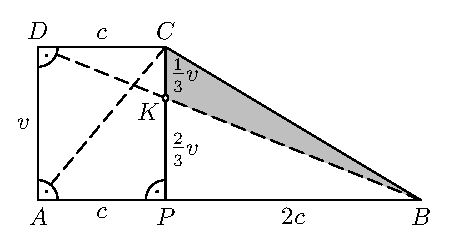
\includegraphics{obrazky/65K3}\\

Obr. 8
\end{center}
Z~predpokladu $S_{APCD} =\frac{1}{2}S_{ABCD}$ vyplýva pre druhú polovicu obsahu $ABCD$ vyjadrenie $\frac{1}{2}S_{ABCD} = S_{PBC}$, takže $S_{APCD} = S_{PBC}$ čiže $cv =\frac{1}{2}|PB|v$, odkiaľ vzhľadom na to, že $v \neq 0$, vychádza $|PB| = 2c$, v~dôsledku čoho $|AB| = 3c$.

Trojuholníky $CDK$ a $PBK$ majú pravé uhly pri vrcholoch $C$, $P$ a zhodné (vrcholové) uhly pri spoločnom vrchole $K$, takže sú podľa vety $uu$ podobné, a to s~koeficientom $|PB| : |CD| = 2c : c = 2$. Preto tiež platí $|PK| : |CK| = 2 : 1$, odkiaľ $|KP| =\frac{2}{3}v$ a $|CK| =\frac{1}{3}v$.

Posudzované obsahy trojuholníkov $ABC$ a $BCK$ tak majú vyjadrenie
$$S_{ABC} = \frac{|AB| \cdot |CP|}{2}=\frac{3cv}{2} \ \ \ \ \text{a} \ \ \ \  S_{BCK} =\frac{|CK|\cdot |BP|}{2}=\frac{\frac{1}{3}v\cdot 2c}{2}=\frac{cv}{3},$$
preto ich pomer má hodnotu
$$\frac{S_{BCK}}{S_{ABC}}=\frac{\frac{1}{3}cv}{\frac{3}{2}cv}=\frac{2}{9}.$$
\textit{Záver.} Trojuholník $BCK$ zaberá $2/9$ obsahu trojuholníka $ABC$.\\
\\
\kom Najkomplexnejšia úloha tohto seminára precvičí študentov v~používaní vlastností podobných trojuholníkov a taktiež vo vyjadrovaní obsahov trojuholníkov pomocou určiteľných hodnôt. Tvorí tak dôstojnú bodku za týmto seminárom.

\subsection*{Domáca práca}
\begin{tcolorbox}[breakable,notitle,boxrule=0pt,colback=light-gray,colframe=light-gray]\ul{10.8} [58-I-2] Pravouhlému trojuholníku $ABC$ s~preponou $AB$ je opísaná kružnica. Päty kolmíc z~bodov $A$, $B$ na dotyčnicu k~tejto kružnici v~bode $C$ označme $D$, $E$. Vyjadrite dĺžku úsečky $DE$ pomocou dĺžok odvesien trojuholníka $ABC$.

\end{tcolorbox}

\rieh Označme odvesny trojuholníka $ABC$ zvyčajným spôsobom $a$, $b$ a protiľahlé uhly $\alpha$, $\beta$. Stred prepony $AB$ (ktorý je súčasne stredom opísanej kružnice) označíme $O$ (obr. 9).

Výška $v = CP$ rozdeľuje trojuholník $ABC$ na trojuholníky $ACP$ a $CBP$ podobné trojuholníku $ABC$ podľa vety $uu$ ($\alpha + \beta = 90^\circ$), úsečka $OC$ je kolmá na $DE$ a navyše $|OC| = |OA| = r$ (polomer opísanej kružnice). Odtiaľ $|\ma OCA| = |\ma OAC| = \alpha$ a $|\ma DCA| = 90^\circ - |\ma OCA| = \beta$.

Pravouhlé trojuholníky $ACP$ a $ACD$ so spoločnou preponou $AC$ sa teda zhodujú aj v~uhloch pri vrchole $C$. Sú preto zhodné, dokonca súmerne združené podľa priamky $AC$. Analogicky sú trojuholníky $CBP$ a $CBE$ súmerne združené podľa $BC$. Takže $|CD|= |CE| = v$, čiže $|DE| = 2v = 2ab/\sqrt{a^2 + b^2}$, lebo z~dvojakého vyjadrenia dvojnásobku obsahu trojuholníka $ABC$ vyplýva $v = ab/|AB|$, pričom $|AB| =\sqrt{a^2 + b^2}$.

\textit{Poznámka.} Namiesto dvojakého vyjadrenia obsahu môžeme na výpočet výšky $CP$ využiť podobnosť trojuholníkov $CBP$ a $ABC$: $\sin \alpha = |CP|/|AC| = |BC|/|AB|$.
\begin{center}
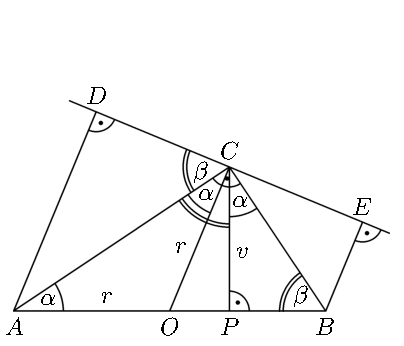
\includegraphics{obrazky/58D21} 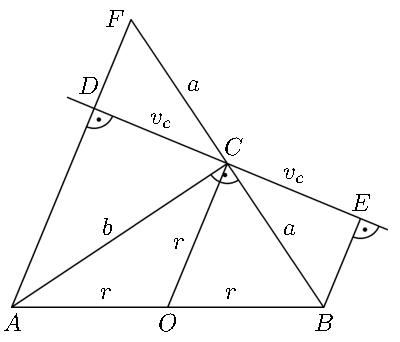
\includegraphics{obrazky/58D22}\\

Obr. 9 \ \ \  \ \ \ \ \ \ \hspace{80pt} \ \ \ \ Obr. 10
\end{center}
\textbf{Iné riešenie.} Úsečka $OC$ je strednou priečkou lichobežníka $DABE$, lebo je rovnobežná so základňami a prechádza stredom $O$ ramena $AB$. Preto $D$ je obrazom bodu $E$ v~súmernosti podľa stredu $C$. Obraz $F$ bodu $B$ v~tej istej súmernosti leží na polpriamke $AD$ za bodom $D$ (obr. 10). Máme $|CF| = |BC| = a$, uhol $ACF$ je pravý, a teda trojuholníky $AFC$ a $ABC$ sú zhodné. Vidíme, že $CD$ je výška v~trojuholníku $AFC$ zhodná s~výškou $v_c$ trojuholníka $ABC$, a $DE$ je jej dvojnásobkom. Veľkosť výšky $v_c$ dopočítame rovnako ako v~predchádzajúcom riešení.

\textit{Záver.} $|DE| = 2ab/\sqrt{a^2 + b^2}$.\\
\\
\begin{tcolorbox}[breakable,notitle,boxrule=0pt,colback=light-gray,colframe=light-gray]\ul{10.9} [58-II-2]
V~pravouhlom trojuholníku $ABC$ označíme $P$ pätu výšky z~vrcholu $C$ na preponu $AB$ a $D, E$ stredy kružníc vpísaných postupne trojuholníkom $APC$, $CPB$. Dokážte, že stred
kružnice vpísanej trojuholníku $ABC$ je priesečníkom výšok trojuholníka $CDE$.

\end{tcolorbox}

\rieh V~pravouhlom trojuholníku $ABC$ s~preponou $AB$ označme $\alpha$ veľkosť vnútorného uhla pri vrchole $A$, zrejme potom platí $|\ma ACP| = 90^\circ -\alpha, |\ma PCB| = \alpha.$ Stred $D$ kružnice vpísanej trojuholníku $APC$ leží na osi uhla $PAC$, takže $|\ma DAC| = \frac{1}{2}\alpha$, a podobne aj $|\ma PCE| = \frac{1}{2}\alpha$. Odtiaľ pre veľkosť uhla $AUC$ v~trojuholníku $AUC$, pričom $U$ je priesečník polpriamok $AD$ a $CE$ (obr. 11), vychádza
$$|\ma AUC| = 180^\circ -\bigg(90^\circ -\alpha + \frac{1}{2}\alpha\bigg) -\frac{1}{2}\alpha = 90^\circ.$$
To znamená, že polpriamka $AD$ je kolmá na $CE$, úsečka $DU$ je teda výška v~trojuholníku $DEC$. Úplne rovnako zistíme, že aj polpriamka $BE$ (ktorá je zároveň osou uhla $ABC$) je kolmá na $CD$. Dostávame tak, že priesečník polpriamok $AD$ a $BE$, čo je stred kružnice vpísanej trojuholníku $ABC$, je zároveň aj priesečníkom výšok trojuholníka $DEC$.
\begin{center}
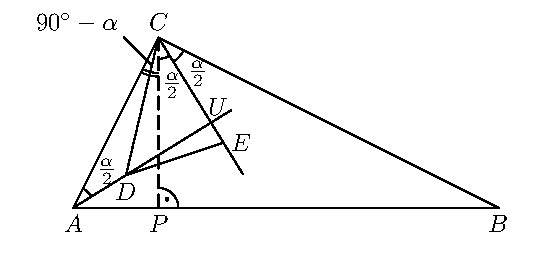
\includegraphics{obrazky/58K21}\\

Obr. 11
\end{center}
\textbf{Iné riešenie.} Označme $F$ a $G$ zodpovedajúce priesečníky priamok $CD$ a $CE$ so stranou $AB$ (obr. 12). Podľa úlohy vyriešenej na seminári v~škole je trojuholník $CAG$
\begin{center}
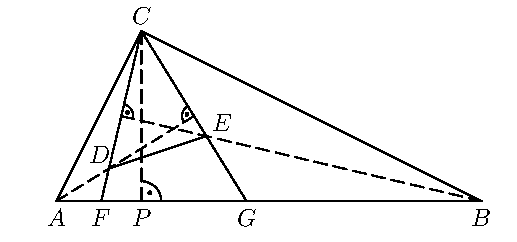
\includegraphics{obrazky/58K22}\\

Obr. 12
\end{center}
rovnoramenný so základňou $CG$. Os $AD$ uhla $CAG$ rovnoramenného trojuholníka $CAG$ je tak aj jeho osou súmernosti, a je preto kolmá na základňu $CG$, teda aj na $CE$. Podobne zistíme, že aj trojuholník $CBF$ je rovnoramenný so základňou $CF$, takže os $BE$ uhla $FBC$ je kolmá na $CF$, teda aj na $CD$. Priesečník oboch osí $AD$ a $BE$ je tak nielen stredom kružnice vpísanej trojuholníku $ABC$, ale aj priesečníkom výšok trojuholníka $CDE$, čo sme mali dokázať.

\subsection*{Doplňujúce zdroje a materiály}
Vhodným doplnkom nielen tohto, ale všetkých ďalších geometrických seminárov je publikácia [~\cite{andreescu2013}], ktorá obsahuje veľké množstvo riešených úloh z~euklidovskej geometrie, od jednoduchých až po úroveň medzinárodných súťaží.

\url{https://old.kms.sk/~mazo/matematika/pocitanieUhlov.pdf}

